%=====================================================================%
% DOCUMENT DEFINITION
%=====================================================================%

\documentclass[12pt]{article}

\usepackage[english]{babel}

\usepackage{subcaption}

\usepackage{gensymb}

\usepackage{setspace}
\onehalfspacing

\usepackage[
    a4paper,
    top=2cm,
    bottom=2cm,
    left=2cm,
    right=2cm,
    marginparwidth=1.75cm
]{geometry}

\usepackage[skip=8pt plus1pt, indent=20pt]{parskip}

% inserting images
\usepackage{graphicx}
\usepackage{float}
\graphicspath{{images/}}

% references
%\usepackage{csquotes}
%\usepackage[
    %backend=biber,
    %style=numeric-comp,
    %sorting=none
%]{biblatex}
%\addbibresource{references.bib}

% math
\usepackage{amsmath}
\usepackage{empheq}

% tables
\usepackage{booktabs}

% color
\usepackage{xcolor}

% dummy text
\usepackage{lipsum}


%=====================================================================%
% DOCUMENT
%=====================================================================%
\setlength{\parindent}{0pt} 


\begin{document}

%=====================================================================%
% TITLE PAGE
%=====================================================================%

\begin{titlepage}

\centering
\singlespacing

% ------------------------------------------------
% UNIVERSITY LOGO
% ------------------------------------------------

\includegraphics[width=0.70\textwidth]{bmelogo.png}

\vspace{0.4cm}

{\Large\bfseries
Budapest University of Technology and Economics\par}

\vspace{0.15cm}

{\Large Faculty of Natural Sciences\par}

% ------------------------------------------------
% TITLE
% ------------------------------------------------

\vspace{3.3cm}

{\LARGE\bfseries
M2 - Basic connections for \\
operational amplifiers\par}

\vspace{0.3cm}

{\Large Lab report\par}

% ------------------------------------------------
% DATE
% ------------------------------------------------

\vspace{2.6cm}

{\Large 21/10/2026\par}

% ------------------------------------------------
% LAB RESPONSIBLE
% ------------------------------------------------

\vspace{2.5cm}

{\Large
\underline{Lab responsible}\\[-0.05cm]
\textbf{Viktor Farkas}
\par}

% ------------------------------------------------
% STUDENTS
% ------------------------------------------------

\vfill

\begin{minipage}[t]{0.47\textwidth}
    \centering

    {\Large {Student}\par}

    \vspace{0.1cm}

    {\bfseries
    Abigél ORTUTAY (UGHRKC)\par}
     {\normalsize
    Physics-engineering BSc 3rd year\par}
    {\normalsize
    abico.ortutay@gmail.com}
    
\end{minipage}
\hfill
\begin{minipage}[t]{0.47\textwidth}
    \centering

    {\Large {Student}\par}
   

    \vspace{0.1cm}

    {\bfseries
    Hanna ERTL (SPH4U7)\par}
    {\normalsize
    Physics-engineering BSc 3rd year\par}
    {\normalsize
    hannavedaertl@gmail.com}
    
    
\end{minipage}

\vspace{1.3cm}

\end{titlepage}


%=====================================================================%
% REPORT STARTS HERE
%=====================================================================%
\begin{abstract}
    \noindent 
\end{abstract}

\section{Theoretical introduction} 
This measurement focused on the operational amplifiers (opamps). Different configurations of these opamps, result in various applications, such as a voltage or current amplifier, both inverting and non inverting modes, voltage follower (also known as buffer), adder and subtractor, and integration and differentiator circuits.

The basic operation of an opamp relies on the potential difference between its inputs. This potential difference is multiplied by some gain factor to result in the output voltage. It follows the equation: U$_{out}$ = A$_u\cdot$(U$_1$ - U$_2$). \\ With U$_1$ and U$_2$ being the voltages at the non-inverting and inverting inputs, respectively.

The basic configurations of the opamp mentioned above rely on the basis of being inverting or non-inverting. The differentiation between the two modes is the input signal of the opamp. If the input voltage is fed into the negative (inverting) input then the input signal will be negatively multiplied resulting in an output of the opposite sign. On the non-inverting (positive) input, the sign of the output voltage will be analogous to that of the input voltage. The amplitude of the opamp is configured by the ratios of the resistances of the circuit, with a resistor on the inverting input R$_s$ and a feedback resistor R$_v$.

Amplification of inverting amplifier: $A_u=-\left( \frac{R_v}{R_s} \right)$

Amplification of non-inverting amplifier: $A_u=1+\left( \frac{R_v}{R_s} \right)$

The opamp requires a power supply. Upon saturation, when the opamp reaches its absolute maximum amplification gain, the output voltage saturates to the positive or negative supply voltage, depending on the circuitry being an inverting or non-inverting amplifier. There is a linear region of amplification before the saturation, in this region the output directly follows the input differential voltage equation shown above. However, upon saturation this linearity ceases, the output voltage caps, it shows a cut off when the input differential exceeds the threshold limit, this is what we refer to as the saturation of the signal.

Often we calculate with ideal opamps as real opamps have many factors and parasitic qualities which make calculations incredibly tiresome and very tedious, for the ideal opamps we assume an infinite input resistance and zero output resistance, with infinite bandwidth and common mode rejection, another assumption which simplifies calculation is the virtual ground assumption in the negative feedback linear mode. To near these ideal conditions, real opamps have input resistances in the M$\Omega$ magnitudes, open loop gains (amplifications) near millions, and output resistances of just a few $\Omega$s.
Our laboratory configurations don't approach these ideals as such, our setup is detailed in the section: Measurement setup below.

In the adder (summing) circuit the operation is to output a voltage that is a weighted sum of the multiple input voltages lead through the resistors, driven all through the inverting input of the opamp. In this case the node equation gives us an output voltage of:

$\frac{U_1}{R_1}+\frac{U_2}{R_2}+\frac{U_3}{R_3}+\frac{U_{out}}{R_v}=0$

$U_{out}= -\left( \frac{R_v}{R_1} U_1+\frac{R_v}{R_2} U_2+\frac{R_v}{R_3} U_3\right)$

The subtractor circuit purely uses the potential difference between the input voltages on both inverting and non-inverting input, no open loop gain or resistors affect the output voltage in the case of the subtractor circuit:

$U_{out}= U_{in1} - U_{in2}$

The voltage follower - also known as buffer - circuit has the aim of achieving unity gain, in reality we often achieve near unity gain $A_u\approx1$. The purpose of this opamp is to provide low-impedance voltage drive to following loads from an initial high input impedance signal source.

Differentiator circuits place a capacitor between the input and feedback resistor on the amplifier, introducing an RC constant for accuracy in the equation of the output voltage, resulting in a phase shift between input and output signals. The original purpose however is to produce an output signal proportional to the rate of change of the input voltage, this protects the load from any steep changes in the input voltage, a great use in control engineering.

$U_{out}= -CR_v \frac{dU_{in}(t)}{dt}$

Integrator circuitry swaps the positions of the resistor and capacitor. This is widely used in instruments such as radiation dose integration from pulse counts. The RC time constant appears again for accuracy in integration, resulting in the output relationship:

$U_{out}= -\frac{1}{R_sC}\int_{0}^{t}U_{in}dt$

The Miller effect appears in the high frequency range where it reduces the amplification by the parasitic stray capacitance which arises between the inverting input and output, multiplied by the stage gain:

$C_{eff}=C\left( 1+A \right)$

\section{Measurement tools}
For this measurement, we used the following list of tools:
\begin{itemize}
\item OK Industries Inc. CM-140 L breadboard
\item ST $\mu$A741CN operational amplifier - 93d427
\item Resistors: 470 k$\Omega$ (1 piece), 100 k$\Omega$ (1 piece), 1 k$\Omega$ (4 pieces)
\item Banana plugs (8 pieces)
\item Crocodile clip (6 pieces)
\item Jumping wires (6 pieces)
\item HM 8030-4 HAMEG Function generator
\item HM8040-2 HAMEG Triple power supply
\item HM 8011-3 HAMEG Digital multimeter
\item SIGLENT SDS 1072CML Digital storage oscilloscope
\end{itemize}

\section{Measurement setup}
We configured the circuits shown in the figures by using the breadboard. Following figure 4 for the first task we built the inverting configuration by forming a common ground with the banana cables for all instruments, this way we could set the input voltage and measure the output voltage with respect to this common ground we established. We added a 100 k$\Omega$ resistor to the inverting input pin of the opamp (leg 2) and added the feedback resistor of 470 k$\Omega$ from leg 2 to 6 (output pin).
\begin{figure}[H]
    \centering
    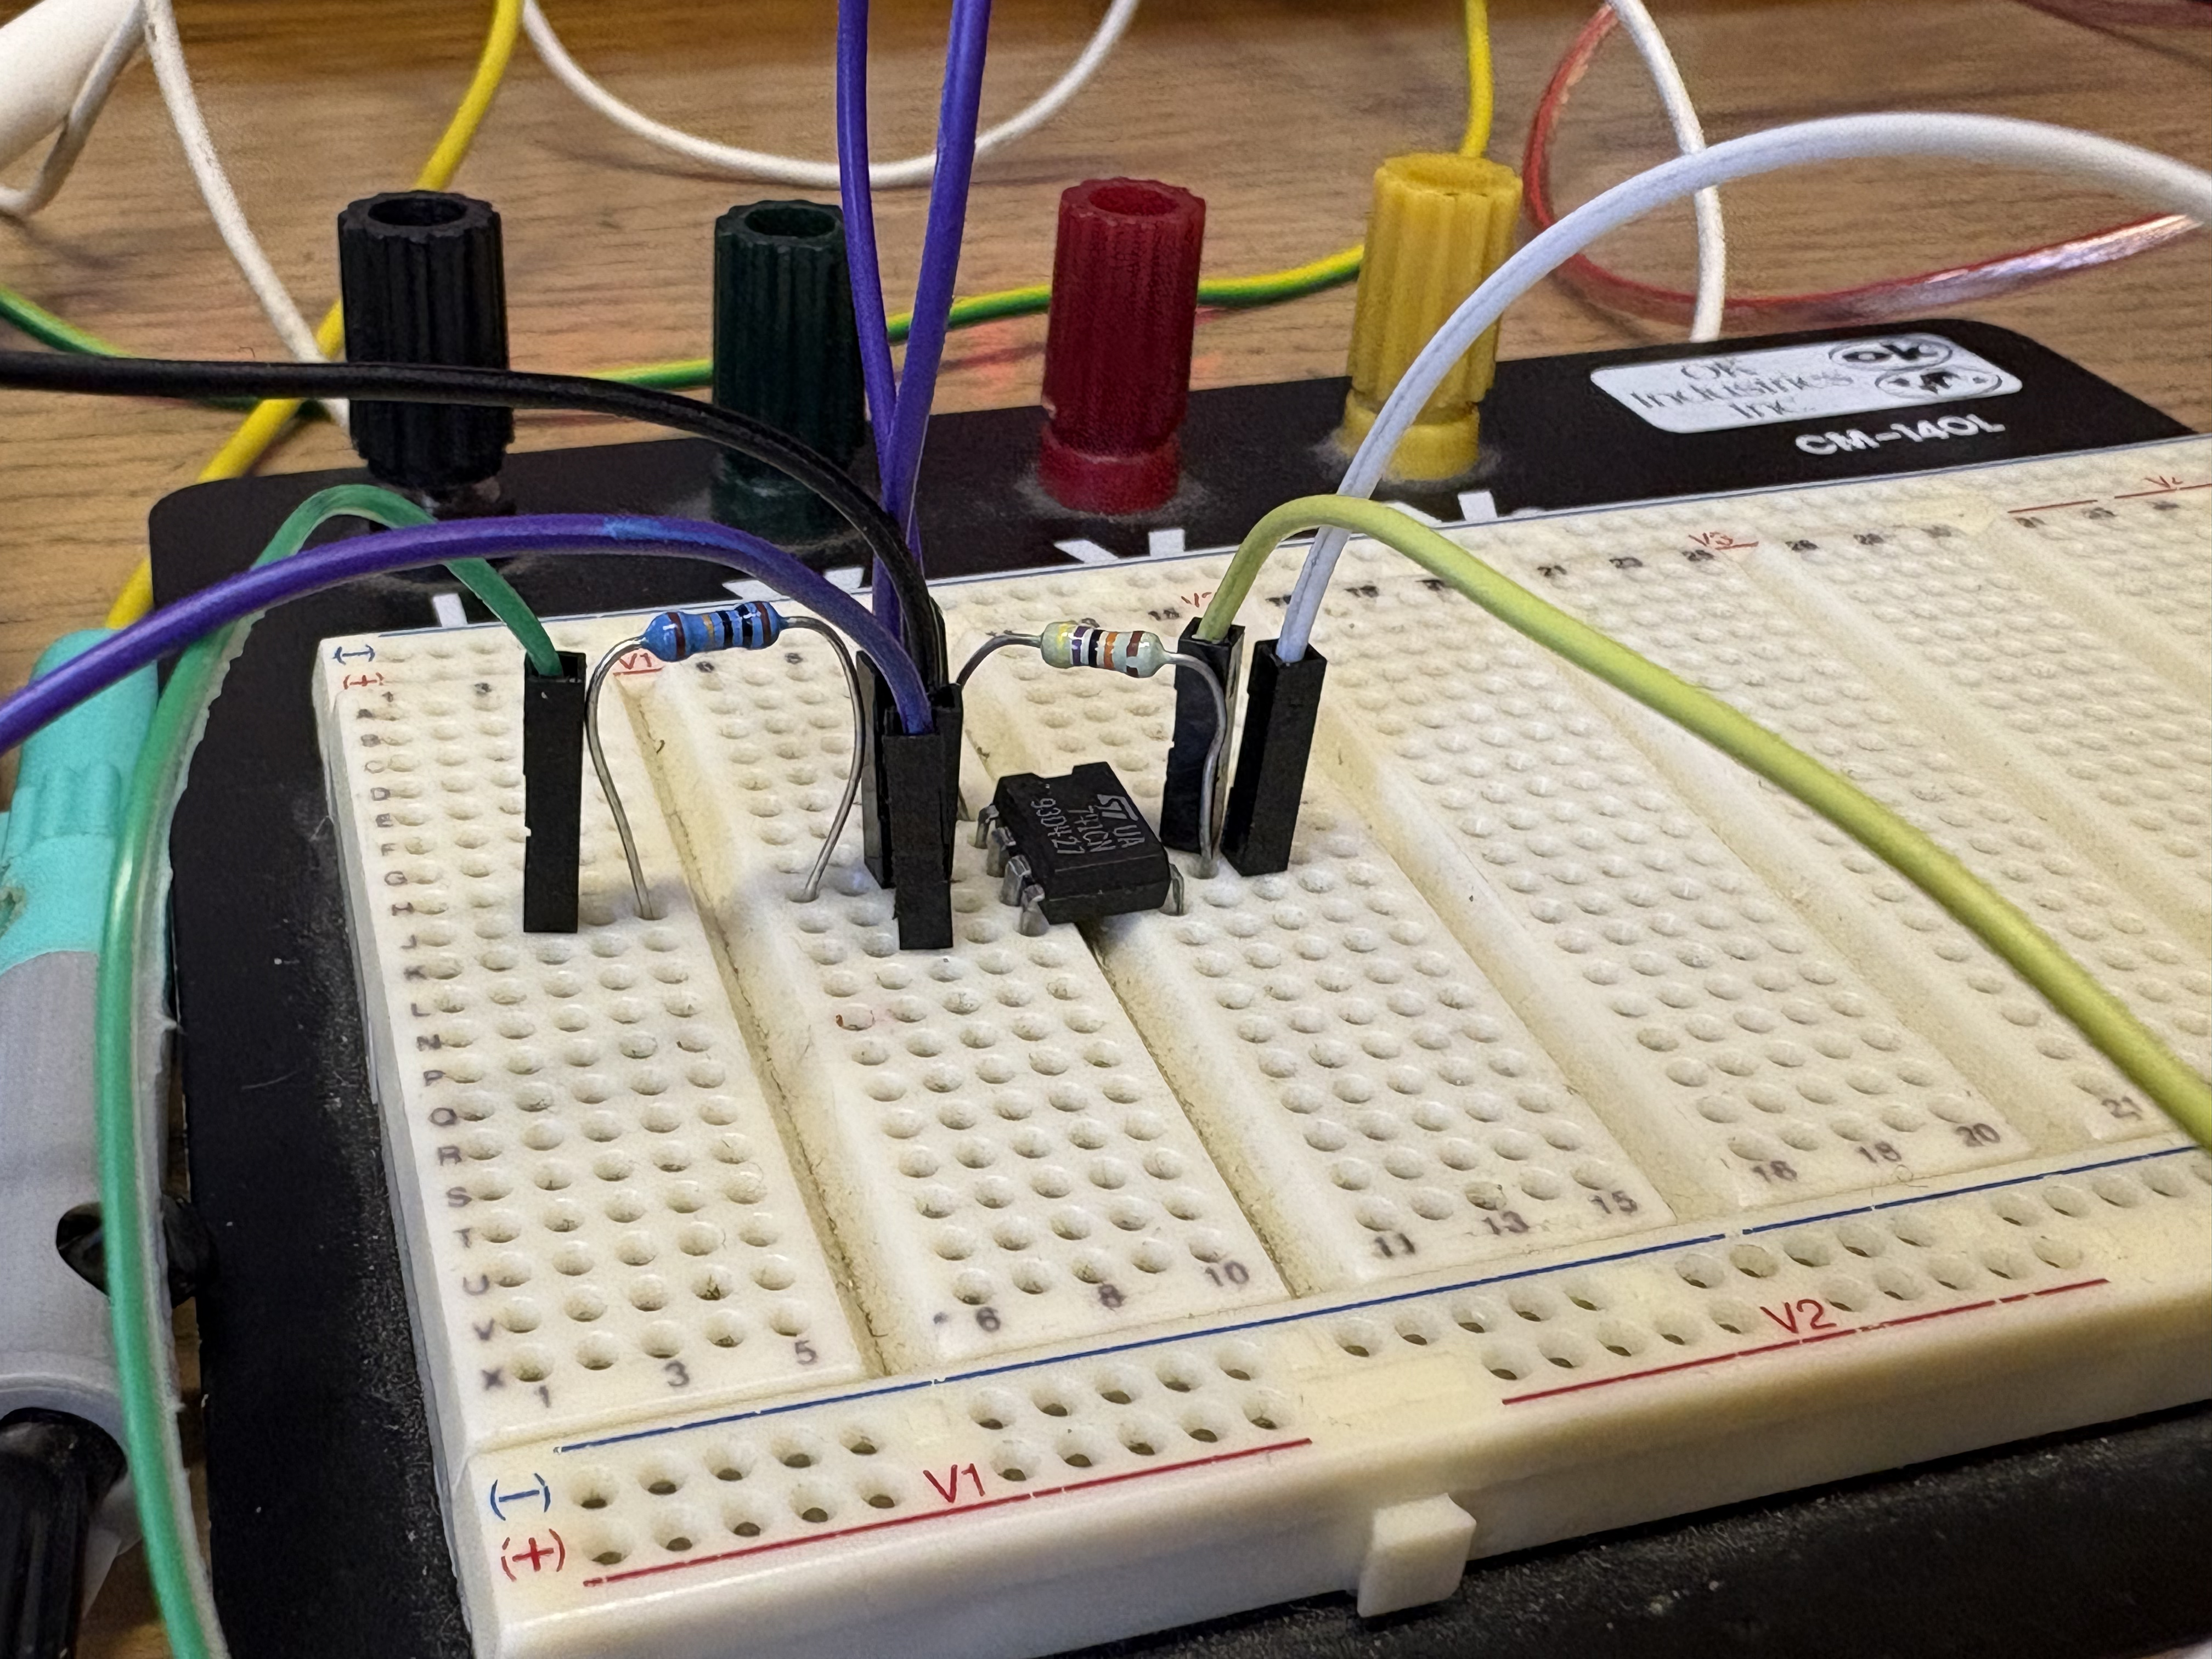
\includegraphics[width=0.7\linewidth]{task1.png}
    \caption{Inverting configuration of task 1}
    \label{fig:task1}
\end{figure}

In task 2 we configured the adder circuit using two additional resistances on the inputs, in this setup all resistors were of the value 1 k$\Omega$. We have to drive both input resistors by the same input voltage, because of this we used one input and connected both resistor legs to simplify the circuitry.

\begin{figure}[H]
    \centering
    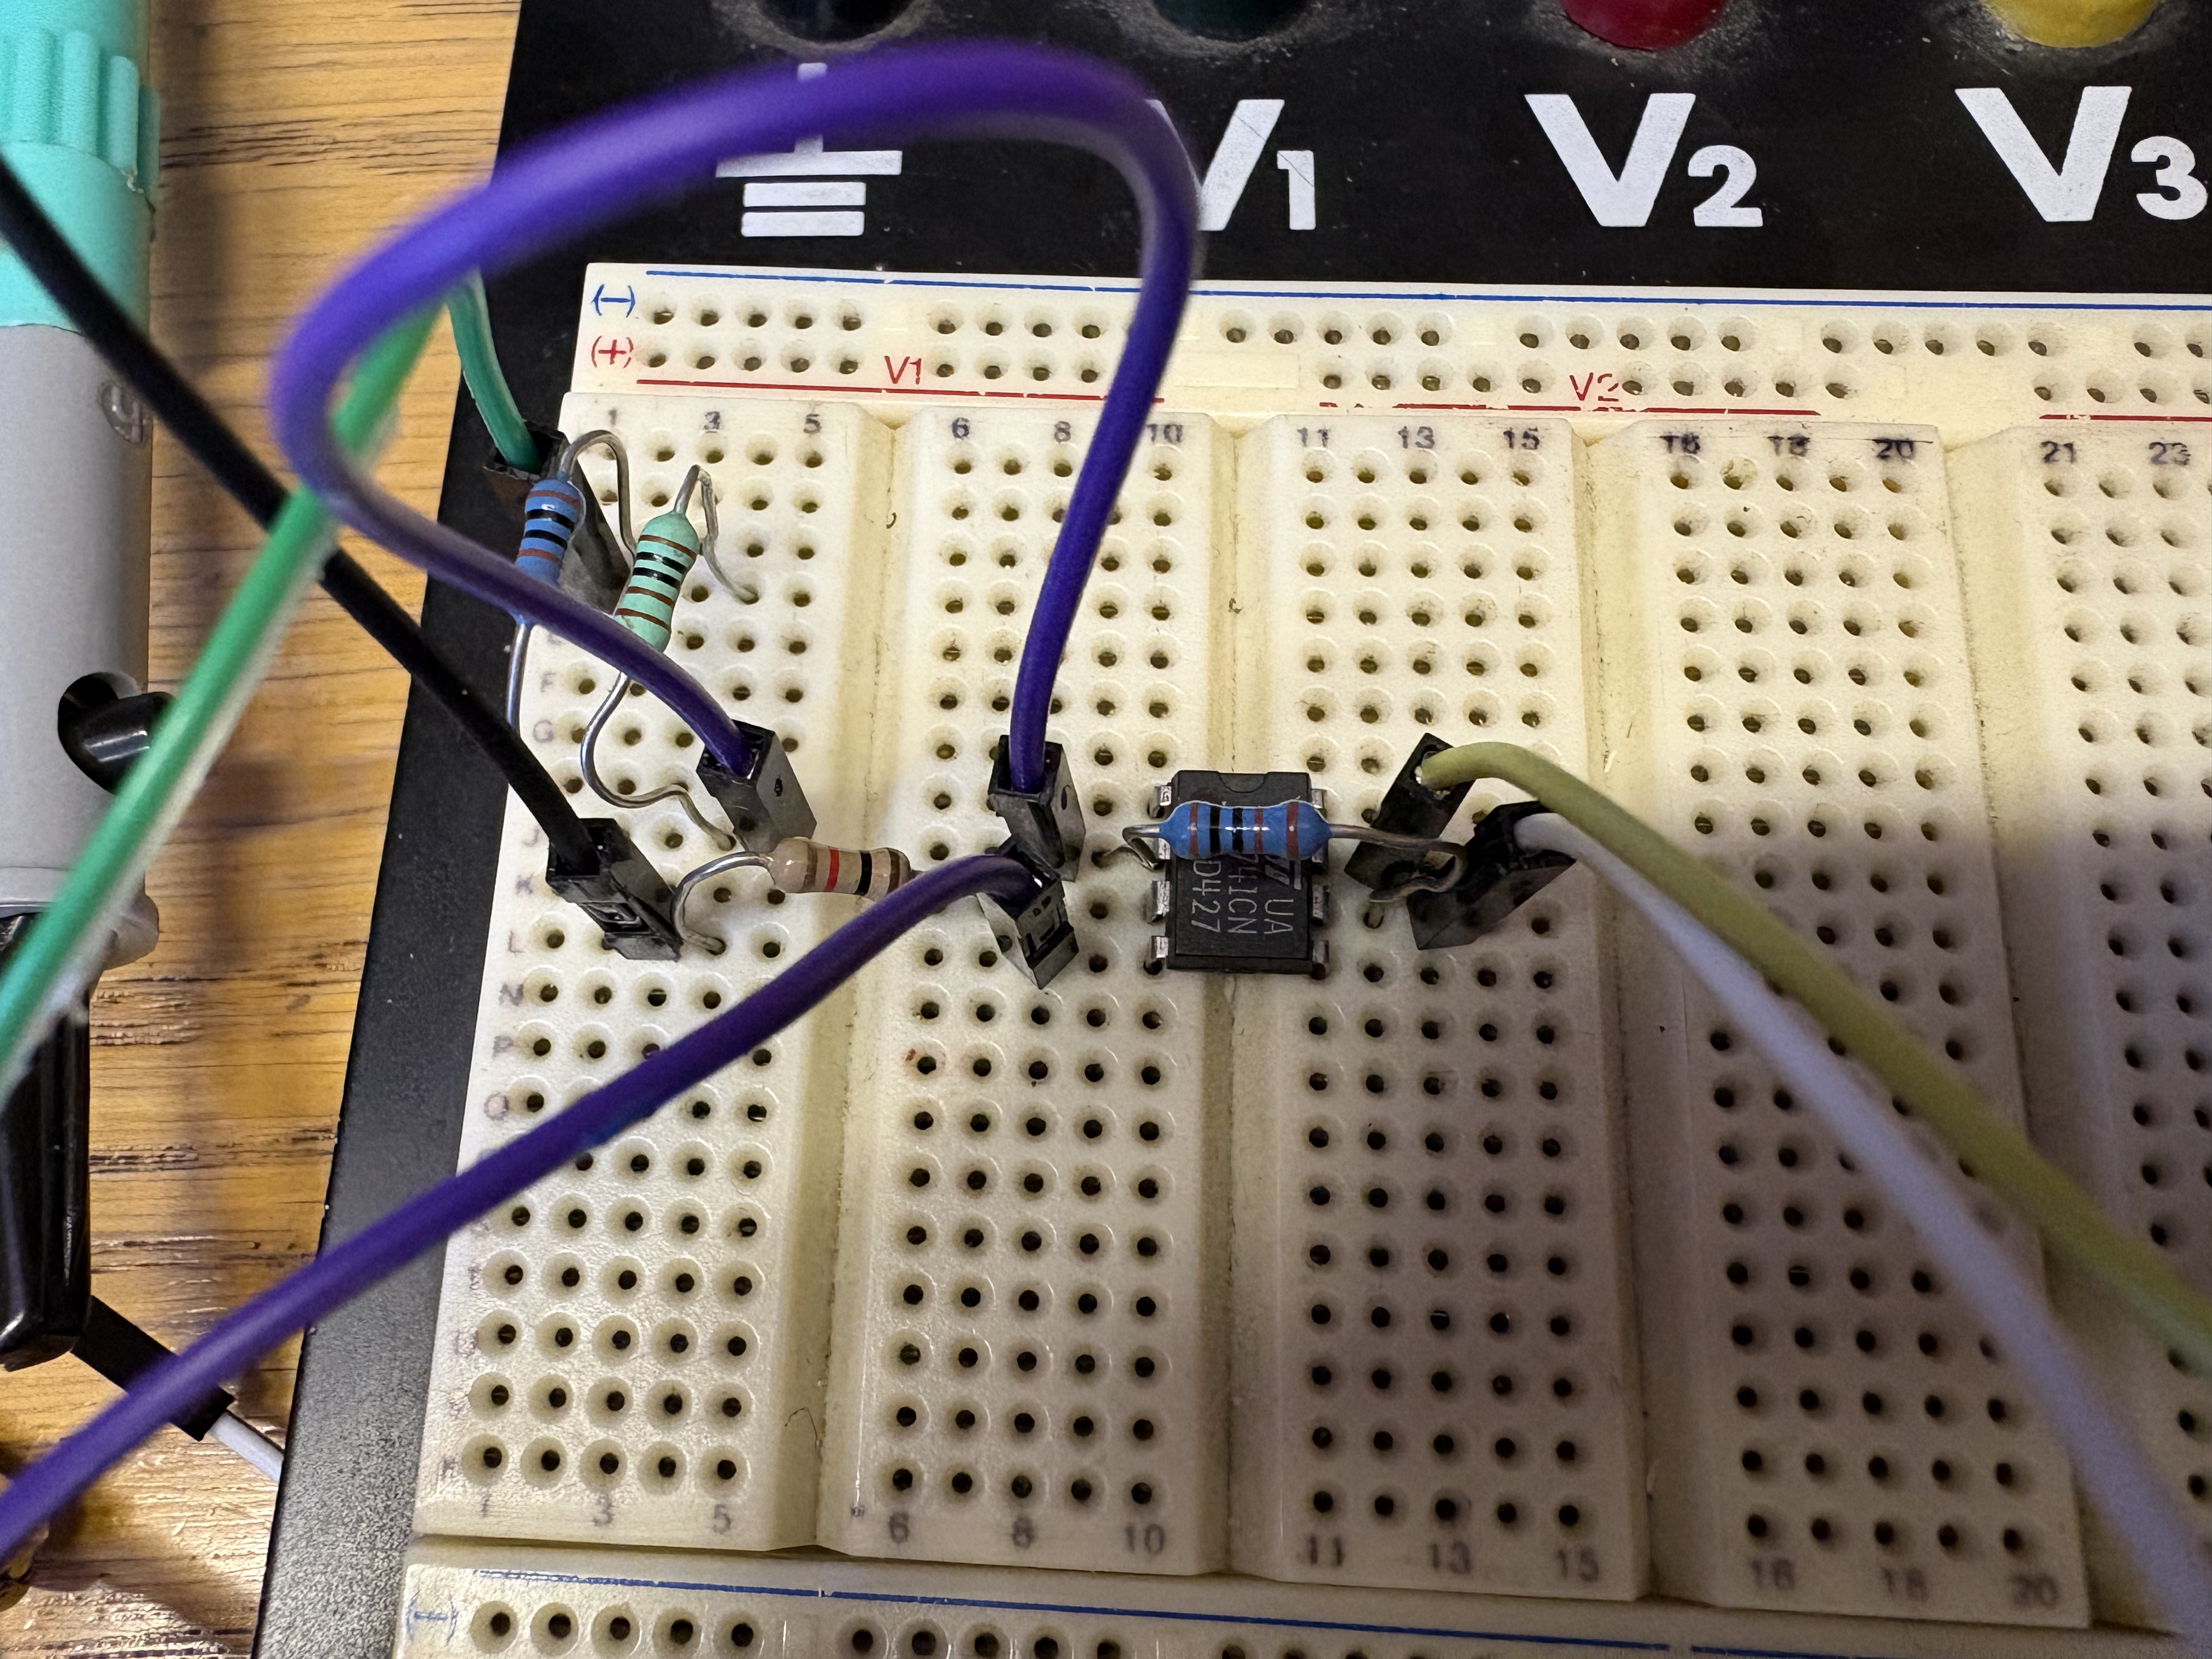
\includegraphics[width=0.7\linewidth]{task2.png}
    \caption{Adder circuit configuration of task 2}
    \label{fig:task2}
\end{figure}

The non-inverting voltage follower of task 3 consisted of only input voltage, output voltage measurement, and the operational amplifier. There were no resistances connected to any pins of the opamp. To achieve this setup we merely connected pin 2 with pin 6 of the opamp to form the feedback loop using one jumping wire, we set a signal driving the circuit through the non-inverting input.

Task 4 called for a differentiator circuit consisting of two capacitances of values $C=10$nF, $C_p=100$pF, and a resistance of value $R_v=100$k$\Omega$. We later removed the capacitance $C_p$ to determine the role it had in the differentiator circuit.
\begin{figure}[H]
    \centering
    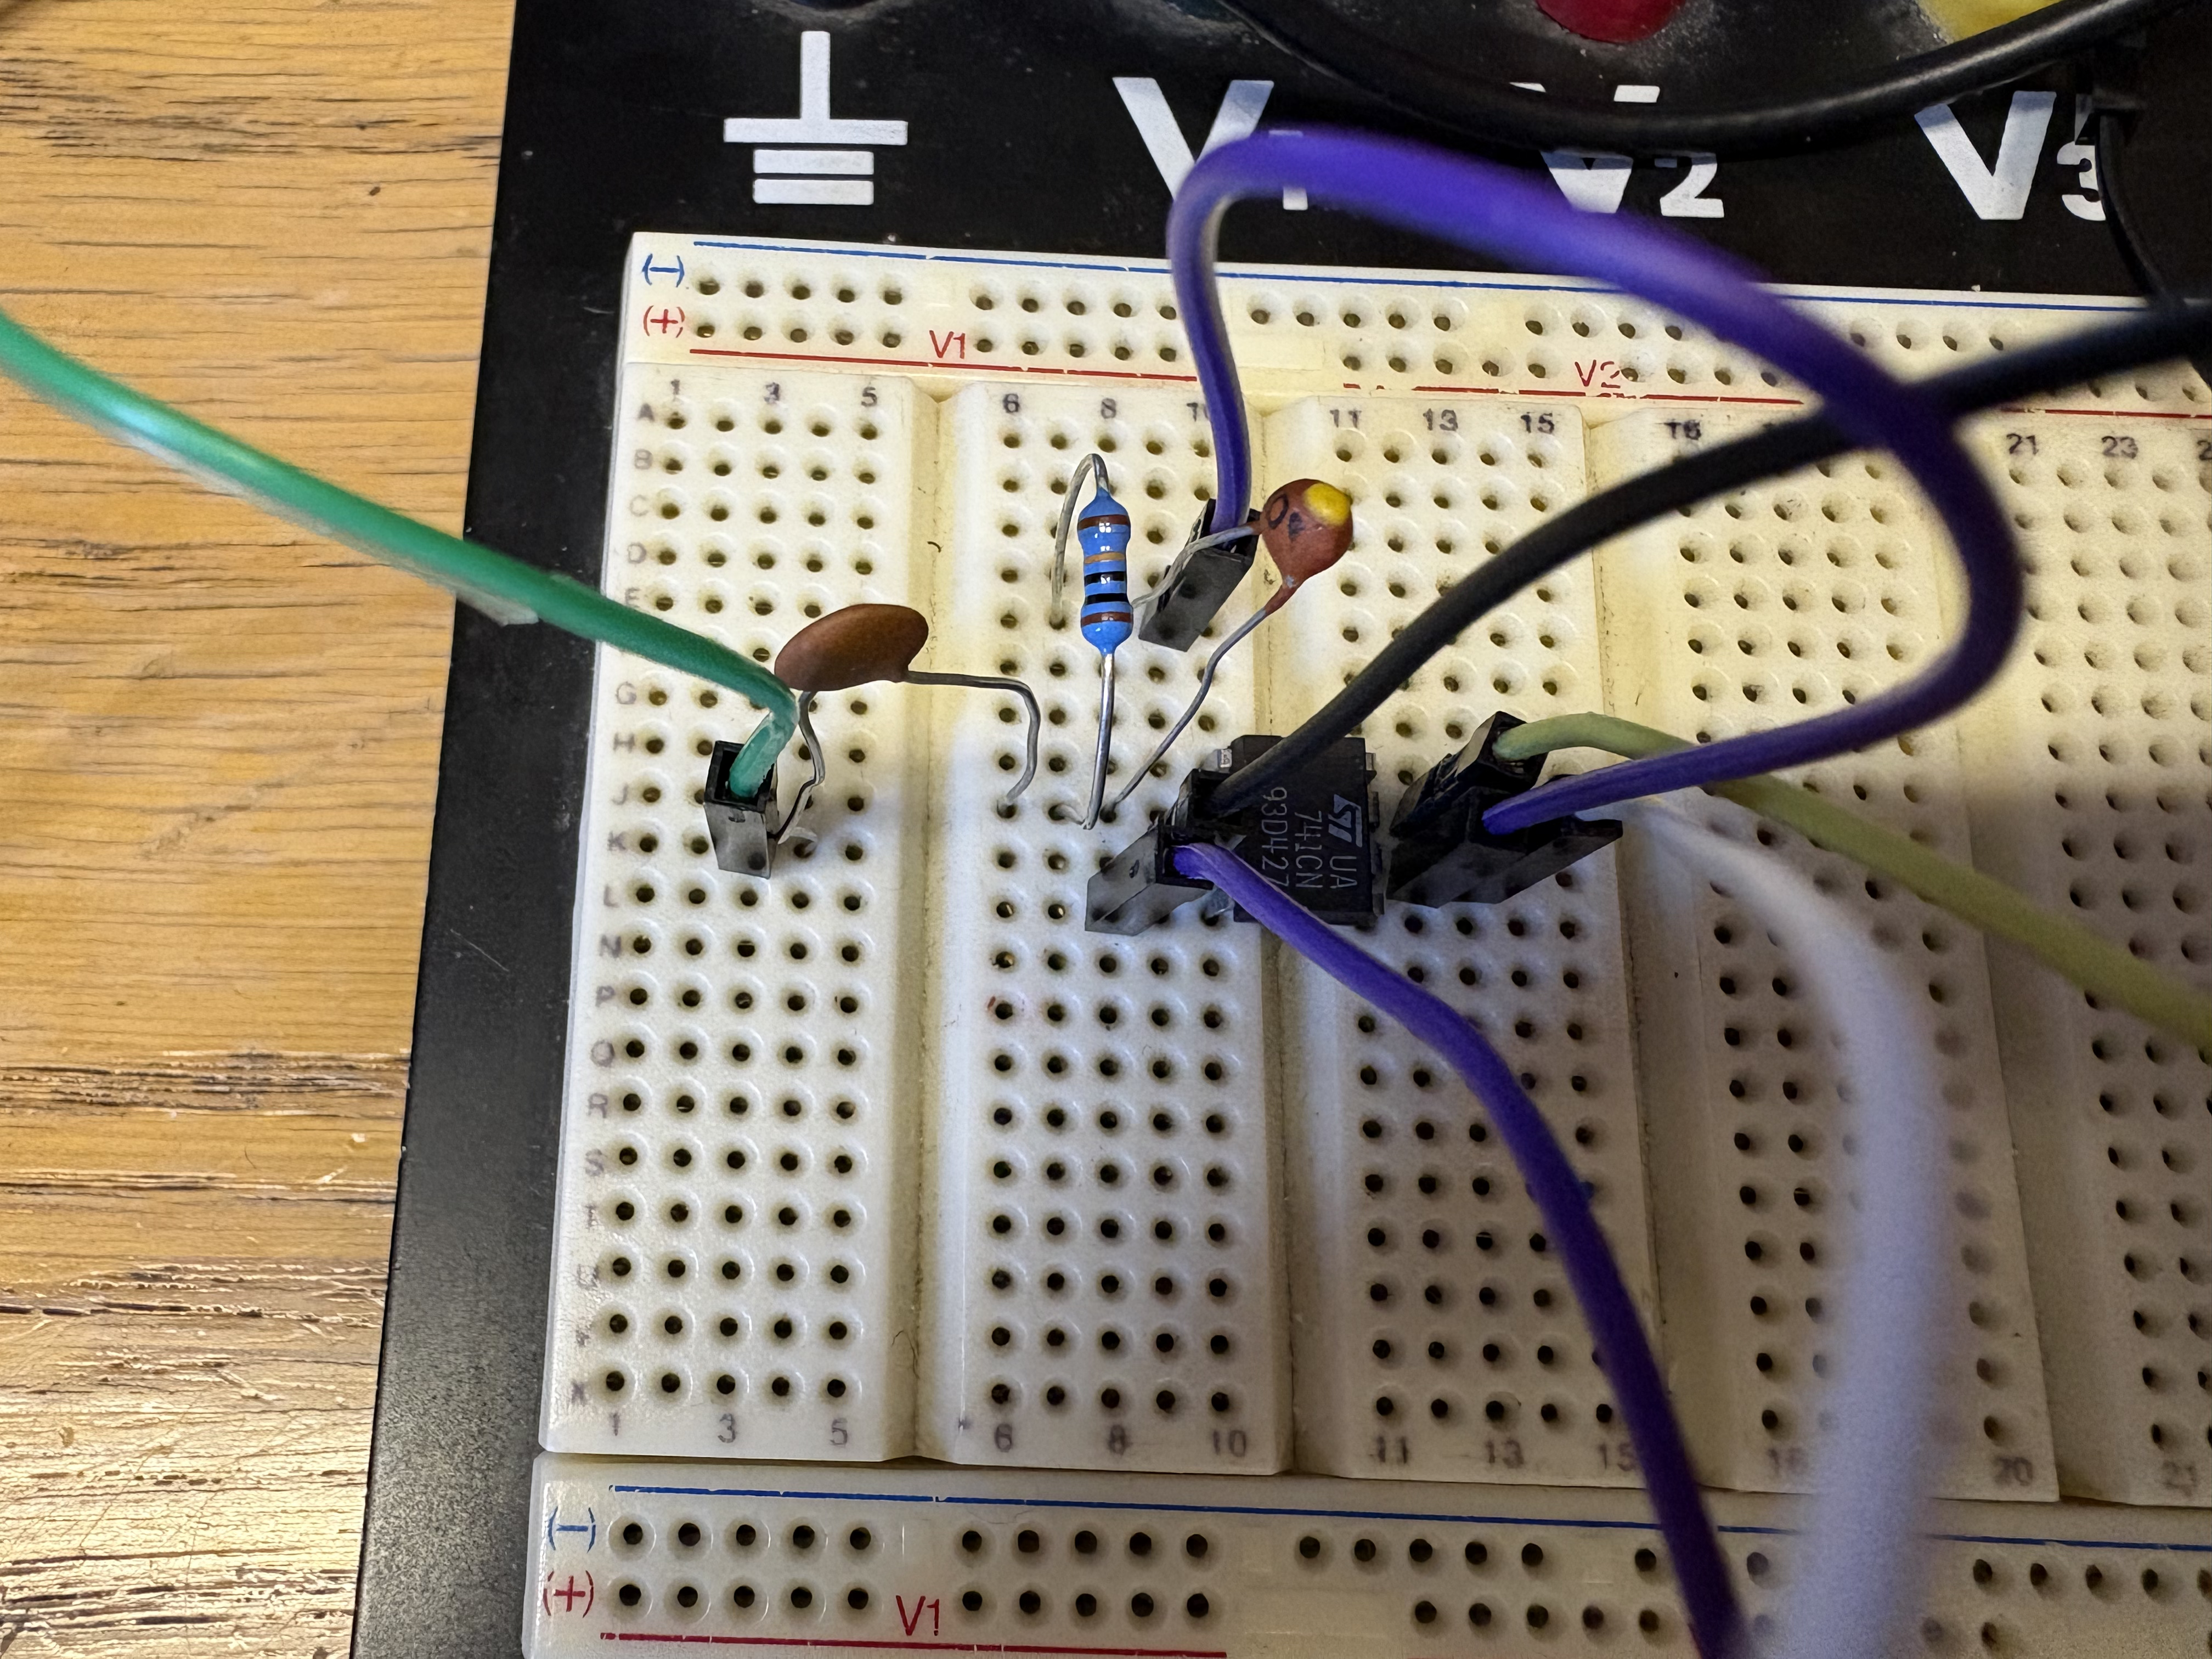
\includegraphics[width=0.7\linewidth]{task4_2.png}
    \caption{Differentiator circuit configuration of task 4}
    \label{fig:task4}
\end{figure}
The integrator circuit was composed similar to the differentiator circuit with the minor change of removing $C_p$ and reordering the resistances as $R_s=100$k$\Omega$ and $R_P=10$M$\Omega$. $R_s$ was connected on the inverting input pin of the opamp while $R_P$ was connected in parallel with C, both connected into the output pin of the opamp. The non-inverting input stayed grounded, as we drove the input voltage through the inverting input. As per the description of the task, we removed to $R_P$ to examine the role it took within the integrator circuit.

\pagebreak\section{Measurements}

\subsection{Saturation voltage of the inverting configuration}
To test the inverting operational amplifier configuration of the $\mu$A741 opamp. We drove a DC input of 500 mV on the inverting input (pin 2) using the power supply instead of the signal generator. We chose this because while the signal generator can supply DC drive theoretically, our lab instructor mentioned that it is not a perfect DC signal and may result in some noise or unwanted artifacts.

Finding the saturation voltage consisted of increasing the input voltage with increments of 100 mV, and determining the position of the cutoff where the output voltage no longer shows an increase as the input is increased.

\begin{table}[H]
    \centering
    \vspace{0.2cm}
    \begin{tabular}{cc}
        \toprule
        $U_{in}$ [V] & $U_{out}$ [V] \\
        \midrule
        0.1 & -0.578 \\
        0.2 & -0.755 \\
        0.3 & -1.145 \\
        0.4 & -1.687 \\
        0.5 & -2.241 \\
        0.6 & -2.626 \\
        0.7 & -3.059 \\
        0.8 & -3.147 \\
        0.9 & -3.147 \\
        1.0 & -3.149 \\
        1.1 & -3.149 \\
        1.2 & -3.149 \\
        \bottomrule
    \end{tabular}
    \caption{Increasing DC input and output voltages of the inverting opamp configuration}
    \label{tab:inverting_dc}
\end{table}

\begin{figure}[H]
    \centering
    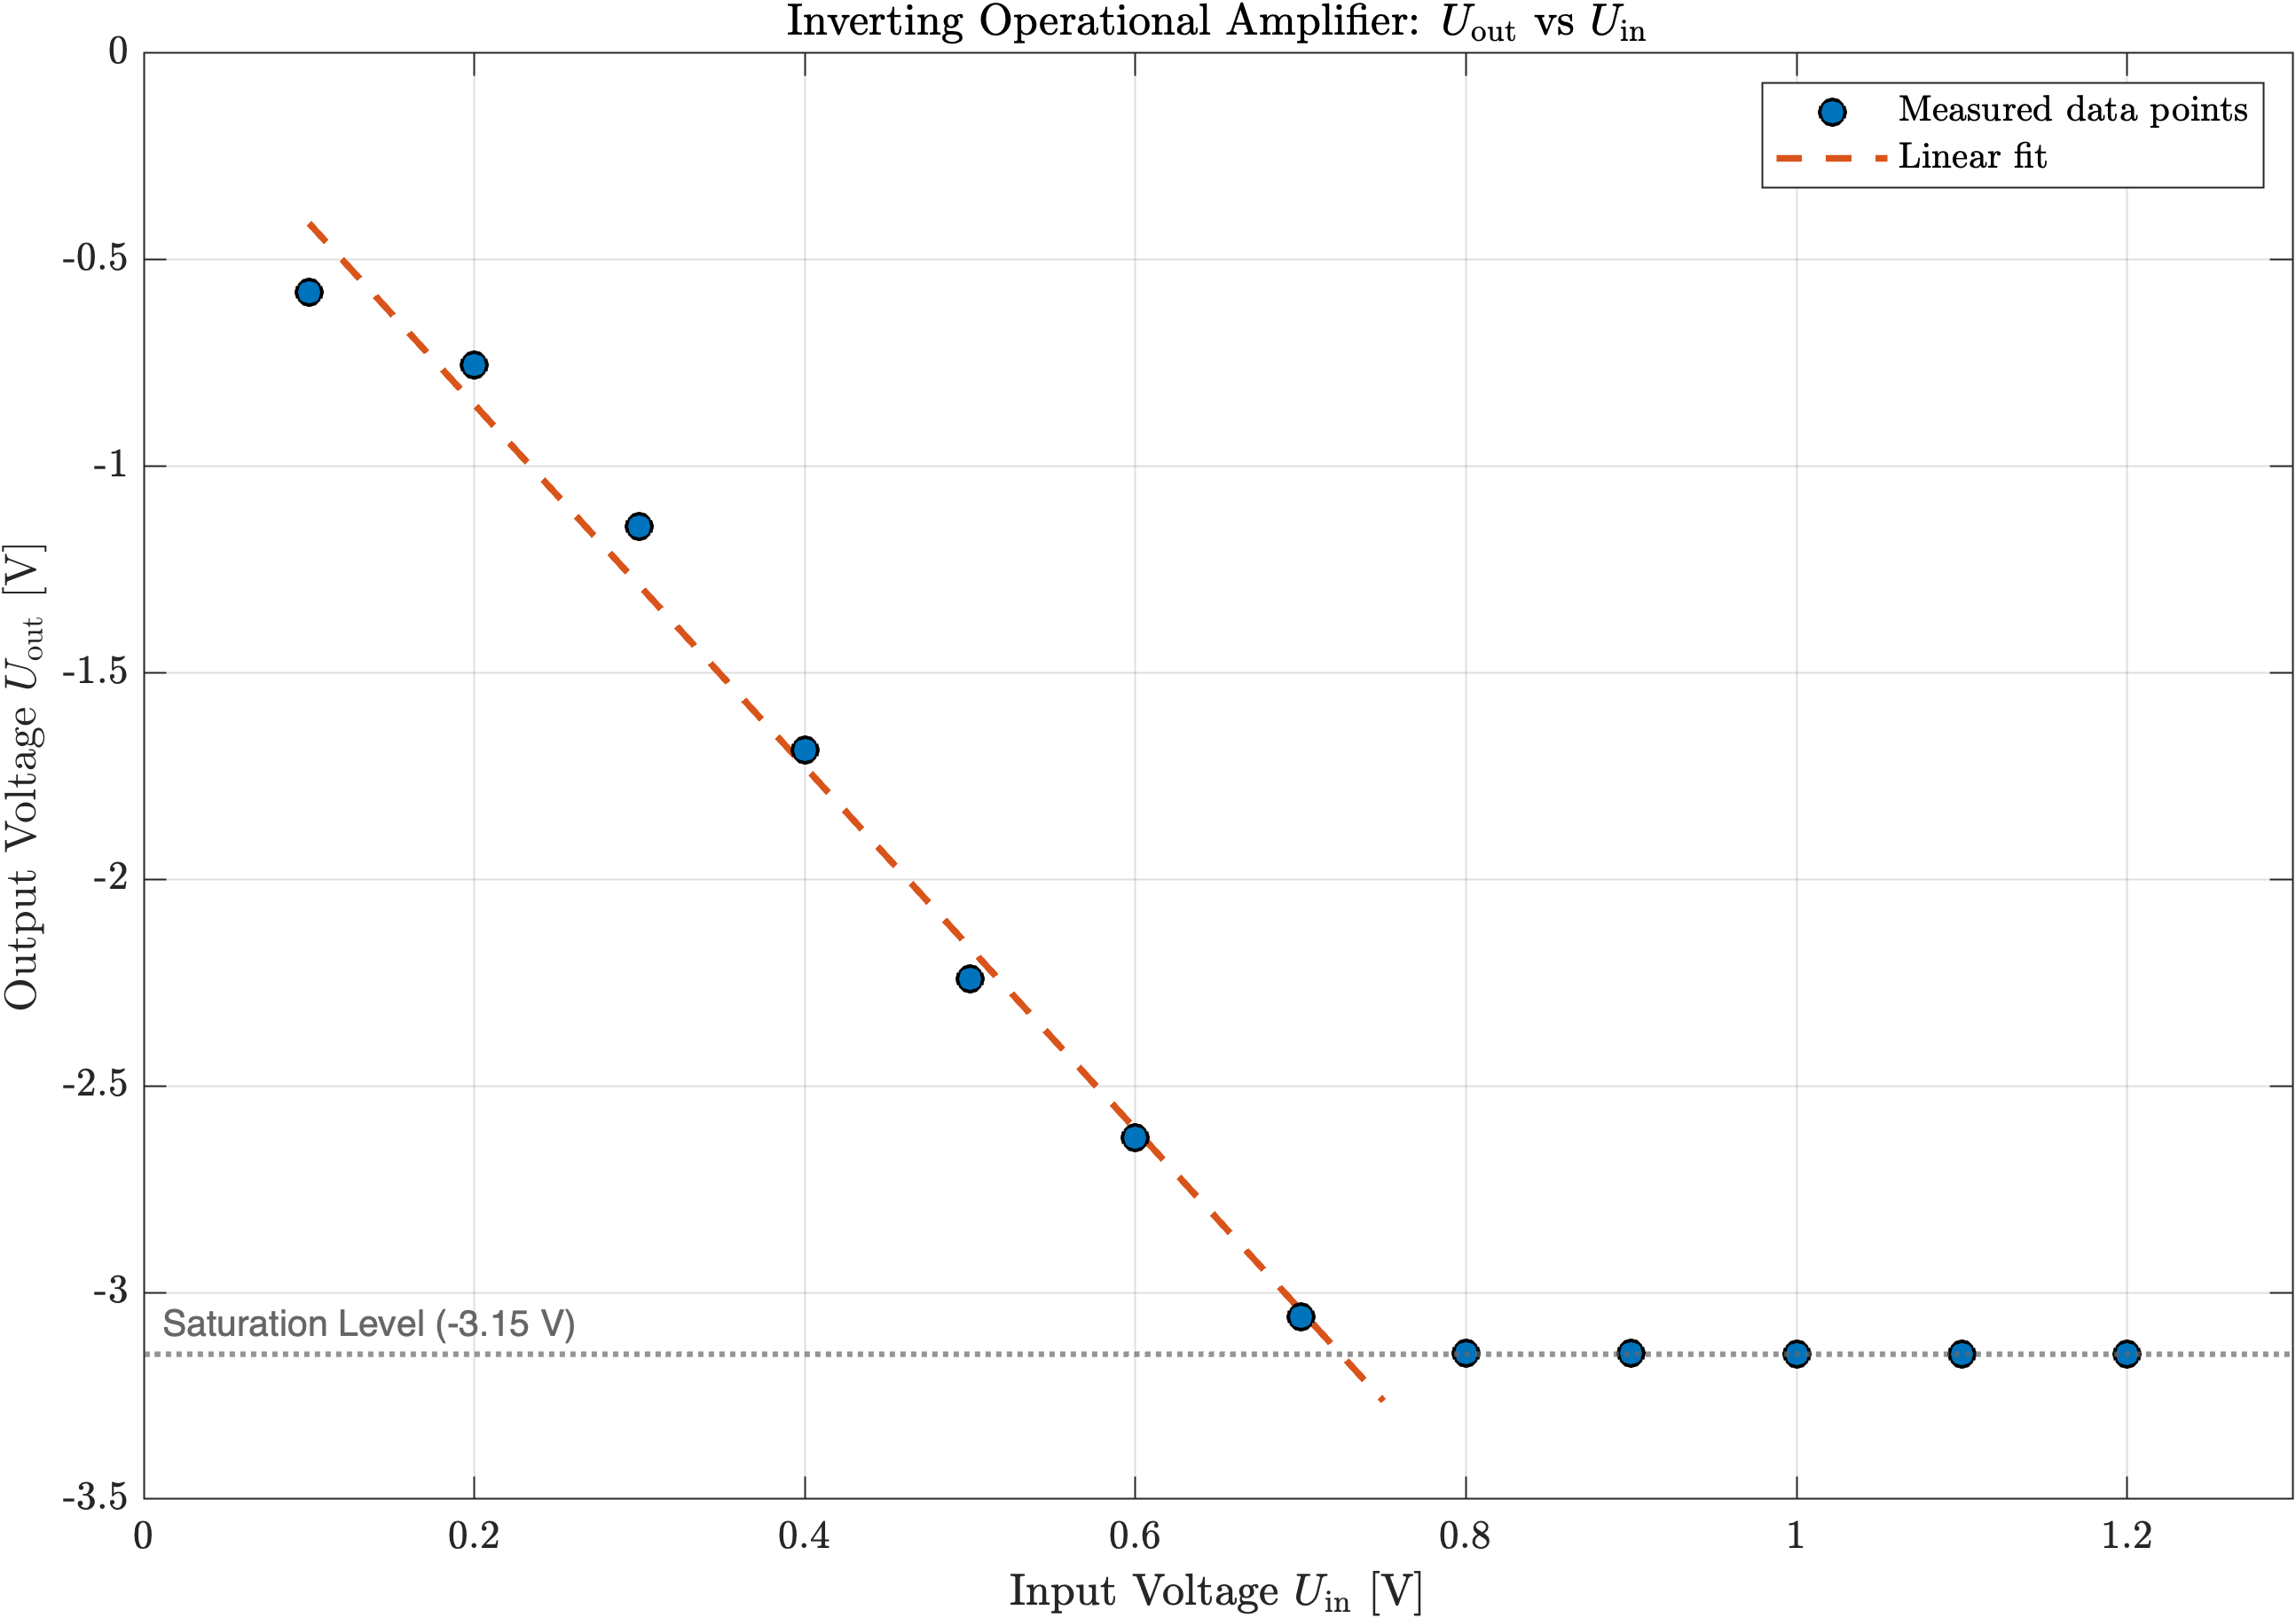
\includegraphics[width=0.7\linewidth]{task1_transfer_curve.png}
    \caption{Finding the saturation voltage of the inverting opamp configuration with DC input}
    \label{fig:task1_transfer_curve}
\end{figure}

We found the saturation voltage to be at $U_{in,sat}=800$ mV, where the output was $U_{out,sat}=-3.137$ V. From this point onwards the output voltage no longer increased with the same increment as previously, hence, here we determine the saturation voltage. Calculating the slope of the fitted line we found an open loop gain of $A_u\approx -4.4$. Theoretically our gain, and hence, relative error should be:

$A_u=-\frac{R_v}{R_s}=-\frac{470 k\Omega}{100 k\Omega} =-4.7$

Relative Error($\%$)$=\frac{4.4-4.7}{4.4}\cdot100\%\approx-6.38\%$

To get a smaller relative deviation we could have measured the true resistance values of the resistors used with a multimeter, as they may have deviated from the theoretical value of 100 k$\Omega$ and 470 k$\Omega$.

\subsection{Operation of the adder amplifier}

\subsection{Non-inverting voltage follower}

\subsection{Operation of the differentiator circuit}

\subsection{Operation of the integrator circuit}

\section{Conclusion}

%\nocite{*}
%\printbibliography 
\end{document}